\documentclass[11pt]{article}
\usepackage[margin=1.1in]{geometry}
\usepackage{booktabs}
\usepackage{graphicx}
\usepackage{amsmath}
\usepackage{setspace}
\usepackage[hidelinks]{hyperref}
\usepackage{natbib}
\bibliographystyle{apalike}
\onehalfspacing

\title{Korea Fama--French Factors:\\An Open Monthly Library with a Verified Construction Pipeline}
\author{Jihwan Woo\thanks{ORCID: 0000-0002-0424-0242. Homepage: \url{https://jihwanw.github.io}. Data and code: \url{https://github.com/jihwanw/korea-fama-french-factors-}, DOI: \href{https://doi.org/10.5281/zenodo.22059320}{10.5281/zenodo.22059320}. This paper describes version 2.0 of the library. Comments and issue reports are welcome. The author thanks the Korean Securities Association community for maintaining open research infrastructure. All errors are my own.}}
\date{August 2026 --- Working Paper}

\begin{document}
\maketitle

\begin{abstract}
\noindent I introduce an open, monthly-updated library of Fama--French five factors plus momentum (MKT--RF, SMB, HML, RMW, CMA, WML) for the Korean stock market, covering July 2001 to the present---the Korean analog of the Ken French Data Library, which does not offer Korea-specific series. Factors are constructed from WRDS Compustat Global security and fundamentals data and Bank of Korea risk-free rates, following \citet{fama1993} and \citet{fama2015} with documented Korean-market adaptations: KOSPI-only breakpoints mirroring the NYSE convention, the 91-day CD rate as the risk-free proxy, and a \citet{shumway1997} delisting-return adjustment. Critically, the construction pipeline is \emph{verified} rather than merely described: applying identical code to US CRSP/Compustat data replicates the official Fama--French factors with correlations of 0.96--0.999. Over 2001--2026, Korea exhibits a significantly positive value premium (HML +0.98\%/month, $t=4.07$) and profitability premium (RMW +0.86\%, $t=3.55$), a \emph{negative} size premium (SMB $-0.25$\%, insignificant), an insignificant investment factor, and a momentum premium (+1.04\%, $t=4.12$) that emerged only after 2000. Each monthly release carries a version DOI for exact reproducibility in citing research.\\[0.5em]
\noindent\textbf{Keywords:} Fama--French factors; Korea; asset pricing; factor library; replication\\
\noindent\textbf{JEL:} G12, G15, C81
\end{abstract}

\section{Introduction}

Empirical asset-pricing research on the US market rests on a piece of shared infrastructure that is easy to take for granted: the Ken French Data Library, which has provided freely downloadable factor returns for more than two decades. A researcher testing a new anomaly, evaluating a fund, or teaching a doctoral seminar does not need to rebuild SMB and HML from raw CRSP data; the community has converged on a common, citable benchmark.

No comparable resource exists for Korea. The French library covers Korea only inside its Asia-Pacific-ex-Japan regional aggregates, which pool Korean stocks with those of Australia, Hong Kong, Singapore, and others; country-level Korean factors must be built by each researcher from commercial databases (FnGuide, DataGuide, or WRDS) whose licenses prohibit redistribution. The predictable consequences are duplicated effort, methodological heterogeneity across studies that is rarely visible to readers, and---because construction choices are seldom fully disclosed---limited reproducibility of Korean asset-pricing results.

This paper introduces an open library that addresses these problems.\footnote{\url{https://github.com/jihwanw/korea-fama-french-factors-}; concept DOI \href{https://doi.org/10.5281/zenodo.22059320}{10.5281/zenodo.22059320}.} Its contributions are threefold in substance, though the third is the one I would emphasize. First, \emph{the data}: six monthly factors (MKT--RF, SMB, HML, RMW, CMA, WML) for the combined KOSPI and KOSDAQ universe from July 2001 to the present---302 months at the time of writing---updated automatically each month, with the risk-free rate and market return provided alongside. Second, \emph{the documentation}: every deviation from the US specification, whether a deliberate market adaptation or a data-driven simplification, is catalogued in a compliance matrix with sensitivity analyses. Third, and most distinctively, \emph{the verification}: rather than asking readers to trust a verbal description of the construction, I apply the identical pipeline code to US CRSP/Compustat data and show that it reproduces the officially published Fama--French factors with correlations between 0.96 and 0.999. Construction validity is demonstrated, not assumed.

Beyond the infrastructure contribution, the library documents four stylized facts about the Korean factor landscape over 2001--2026 that should interest comparative asset-pricing researchers: a strong value premium and a strong profitability premium, a size premium with the ``wrong'' sign, an investment factor indistinguishable from zero, and a momentum premium that is robust in this sample despite the well-known finding of \citet{griffin2003} that momentum was absent in pre-2000 Korean data. I deliberately stop at documentation; causal interpretation of these patterns is left to companion and future work.

The remainder of the paper proceeds as follows. Section~\ref{sec:data} describes the data sources and sample. Section~\ref{sec:construction} details factor construction, including all Korean-market adaptations and simplifications. Section~\ref{sec:verification} presents the US replication test. Section~\ref{sec:landscape} reports the Korean factor landscape and validation results. Section~\ref{sec:usage} explains usage, citation, and the update protocol. Section~\ref{sec:conclusion} concludes.

\section{Data and Sample}\label{sec:data}

\subsection{Security and fundamentals data}

Security-level data come from the WRDS Compustat Global daily security file (\texttt{g\_secd}), restricted to Korean issues (\texttt{fic = KOR}) denominated in Korean won. I retain common shares only (\texttt{tpci = 0}), excluding preferred shares, and issues listed on the Korea Exchange main board (KOSPI, exchange code 248) or KOSDAQ (code 298); the small KONEX venue is excluded. Month-end observations are selected using the file's month-end flag. When a firm has multiple common-share issues in a month, the issue with the largest market capitalization is used. Accounting data come from the Compustat Global fundamentals file (\texttt{g\_funda}) under the standard filters (industrial format, historical standardized data, consolidated statements).

The sample contains 5{,}152 distinct Korean firms with price data beginning January 2000, of which 3{,}861 enter the final panel of 623{,}381 firm-months after the common-share and validity filters. Because Compustat Global retains firms that were subsequently delisted, the sample is free of survivorship bias; Section~\ref{sec:delisting} describes the delisting-return treatment. Fundamentals coverage begins in 1987, comfortably before the price data, and the key accounting fields used here are non-missing for 98--99.9\% of firm-years.

\subsection{Risk-free rate}

The risk-free rate is the 91-day certificate of deposit (CD) yield published by the Bank of Korea (ECOS statistic 721Y001, item 2010000, monthly), the standard proxy in Korean empirical work. Denoting the annualized percentage yield in month $t$ by $y_t$, the monthly rate is the geometric de-annualization
\begin{equation}
r_{f,t} \;=\; \left(1+\frac{y_t}{100}\right)^{1/12} - 1,
\label{eq:rf}
\end{equation}
which is preferred to the arithmetic $y_t/1200$ because it compounds exactly to the quoted annual yield. The CD series is available from March 1991 and therefore never binds the sample start.

\subsection{Sample period}

Factors begin in July 2001. The binding constraint is Compustat Global's Korean price coverage, which starts in 2000: the first June rebalancing that can use December-2000 market equity and fiscal-2000 book equity occurs in June 2001, with returns accruing from July 2001.

\section{Factor Construction}\label{sec:construction}

Construction follows \citet{fama1993} and \citet{fama2015} exactly wherever the Korean data permit. Portfolios are formed at the end of June of year $t$ and held from July of $t$ through June of $t+1$.

\subsection{Notation and variable definitions}

For issue $i$ at the end of month $t$, let $p_{i,t}$ denote the unadjusted close price, $a_{i,t}$ the cumulative adjustment factor for splits and similar corporate actions, $f_{i,t}$ the cumulative total-return factor capturing dividends, and $n_{i,t}$ shares outstanding. The monthly total return is
\begin{equation}
r_{i,t} \;=\; \frac{(p_{i,t}/a_{i,t})\, f_{i,t}}{(p_{i,t-1}/a_{i,t-1})\, f_{i,t-1}} - 1,
\label{eq:ret}
\end{equation}
computed only over consecutive month-ends, and market equity is $ME_{i,t} = p_{i,t}\, n_{i,t}$. The three sorting characteristics for the June-of-year-$t$ formation are
\begin{align}
BM_{i,t} &\;=\; \frac{BE_{i,\,\mathrm{fy}(t-1)}}{ME_{i,\,\mathrm{Dec}(t-1)}}, \label{eq:bm}\\[2pt]
OP_{i,t} &\;=\; \frac{REV_{i} - COGS_{i} - SGA_{i} - INT_{i}}{BE_{i}}\bigg|_{\mathrm{fy}(t-1)}, \label{eq:op}\\[2pt]
INV_{i,t} &\;=\; \frac{AT_{i,\,\mathrm{fy}(t-1)}}{AT_{i,\,\mathrm{fy}(t-2)}} - 1, \label{eq:inv}
\end{align}
where $BE$ is book equity, $\mathrm{fy}(t-1)$ denotes the fiscal year ending in calendar year $t-1$, and $AT$ is total assets. The momentum signal, refreshed monthly, is the formation-window cumulative return
\begin{equation}
MOM_{i,t} \;=\; \prod_{k=2}^{12} (1 + r_{i,t-k}) - 1,
\label{eq:mom}
\end{equation}
which skips month $t-1$ to avoid contamination by short-term reversal \citep{jegadeesh1993}.

\subsection{Timing: why June formation is sufficient for no look-ahead}

Let $\mathcal{F}_\tau$ denote the public information set at date $\tau$, and let $d_i$ be the statutory publication deadline of firm $i$'s annual report. Absence of look-ahead bias requires every accounting input in Eqs.~(\ref{eq:bm})--(\ref{eq:inv}) to satisfy
\begin{equation}
BE_{i,\,\mathrm{fy}(t-1)},\, OP_{i,t},\, INV_{i,t} \;\in\; \mathcal{F}_{\mathrm{Jun}(t)}.
\label{eq:nolookahead}
\end{equation}
In Korea, approximately 95\% of listed firms close their books in December, and the Capital Markets Act requires annual-report filing within 90 days of fiscal year-end, so $d_i \le \mathrm{Mar}(t)$ for the dominant December cohort. June formation therefore guarantees condition~(\ref{eq:nolookahead}) with a slack of at least three months---the same margin the original US design obtains, since US 10-K deadlines also precede the FF June formation by several months.

\subsection{Portfolio assignment and factor definitions}

Let $\mathcal{K}_t$ denote the set of KOSPI (main-board) stocks at the June-$t$ formation. Breakpoints are computed on $\mathcal{K}_t$ only:
\begin{equation}
b^{ME}_t = \mathrm{med}\{ME_{i,t}: i \in \mathcal{K}_t\}, \qquad
b^{X,30}_t,\; b^{X,70}_t = Q_{0.3},\, Q_{0.7}\{X_{i,t}: i \in \mathcal{K}_t\},
\label{eq:breakpoints}
\end{equation}
for each characteristic $X \in \{BM, OP, INV, MOM\}$, and every stock in the full universe (KOSPI and KOSDAQ) is classified against these cutoffs. The rationale mirrors the NYSE convention: if breakpoints were computed on the pooled universe, the roughly $2{:}1$ preponderance of small KOSDAQ issues would drag the size median far below the main-board median, mechanically packing the ``Big'' bucket with mid-caps and blurring the size sort---precisely the distortion \citet{fama1993} avoid by excluding AMEX and NASDAQ from breakpoints.

The value-weighted return of a portfolio $P$ in month $t$ uses lagged market equity as weights:
\begin{equation}
r_{P,t} \;=\; \sum_{i \in P} w_{i,t}\, r_{i,t}, \qquad
w_{i,t} \;=\; \frac{ME_{i,t-1}}{\sum_{j \in P} ME_{j,t-1}}.
\label{eq:vw}
\end{equation}
With six portfolios $\{S,B\}\times\{G,N,V\}$ from the size--$BM$ sort (and analogously $\{W,N,R\}$ for profitability, $\{C,N,A\}$ for investment, $\{L,M,W\}$ for momentum), the factors are
\begin{align}
\mathrm{HML}_t &= \tfrac{1}{2}(r_{SV,t}+r_{BV,t}) - \tfrac{1}{2}(r_{SG,t}+r_{BG,t}), \label{eq:hml}\\
\mathrm{RMW}_t &= \tfrac{1}{2}(r_{SR,t}+r_{BR,t}) - \tfrac{1}{2}(r_{SW,t}+r_{BW,t}), \label{eq:rmw}\\
\mathrm{CMA}_t &= \tfrac{1}{2}(r_{SC,t}+r_{BC,t}) - \tfrac{1}{2}(r_{SA,t}+r_{BA,t}), \label{eq:cma}\\
\mathrm{WML}_t &= \tfrac{1}{2}(r_{SW,t}+r_{BW,t}) - \tfrac{1}{2}(r_{SL,t}+r_{BL,t}), \label{eq:wml}
\end{align}
where the momentum sort in Eq.~(\ref{eq:wml}) is refreshed monthly while Eqs.~(\ref{eq:hml})--(\ref{eq:cma}) hold their June assignment for twelve months. The five-factor SMB averages the small-minus-big legs of the three annual sorts,
\begin{equation}
\mathrm{SMB}_t = \frac{1}{3}\sum_{X \in \{BM,\,OP,\,INV\}} \Bigl[ \tfrac{1}{3}\!\!\sum_{c\,\in\,\text{cols}(X)}\!\! r_{S c,t} \;-\; \tfrac{1}{3}\!\!\sum_{c\,\in\,\text{cols}(X)}\!\! r_{B c,t} \Bigr],
\label{eq:smb}
\end{equation}
and the market factor is the value-weighted return of the full universe in excess of Eq.~(\ref{eq:rf}), $\mathrm{MKT\text{--}RF}_t = r_{M,t} - r_{f,t}$ with $r_{M,t}$ computed as in Eq.~(\ref{eq:vw}) over all sample stocks.

\subsection{Korean-market adaptations}

Four choices adapt the specification to Korean institutions; each follows what I take to be the emerging convention in the international literature.

\emph{KOSPI as the NYSE analog.} Fama and French compute breakpoints from NYSE stocks only, so that the many small NASDAQ issues do not distort the size and characteristic cutoffs. The Korean market has the same two-tier structure: the main board (KOSPI) and the growth venue (KOSDAQ), whose listings outnumber KOSPI's roughly two to one but are far smaller. Size breakpoints are therefore the KOSPI median, and characteristic breakpoints the KOSPI 30th and 70th percentiles; KOSDAQ stocks are classified against these cutoffs, exactly as NASDAQ stocks are classified against NYSE cutoffs.

\emph{CD rate as the T-bill analog.} Korea lacks a continuously traded one-month Treasury bill series over the sample; the 91-day CD yield is the entrenched risk-free proxy in Korean studies.

\emph{June rebalancing under Korean disclosure rules.} Roughly 95\% of Korean listed firms have December fiscal year-ends, and annual reports are due within 90 days, i.e., by the end of March. June formation therefore guarantees at least a three-month gap between statement publication and portfolio use, protecting against look-ahead bias while retaining the exact FF timing.

\emph{Delisting returns.}\label{sec:delisting} CRSP provides delisting returns; Compustat Global does not. Ignoring them truncates each delisted stock's history at its last trading month and overstates portfolio returns. Formally, if $\delta_{i}$ denotes the unobserved return in the delisting month, omitting it biases the value-weighted portfolio return in that month by
\begin{equation}
\Delta r_{P,t} \;=\; w_{i,t}\,\bigl(\hat{\delta} - \delta_i\bigr),
\label{eq:dlbias}
\end{equation}
where $\hat{\delta}$ is whatever the researcher implicitly assumes (zero, under truncation). Using the security file's deletion metadata, I identify 1{,}668 delisted Korean securities and classify deletion reasons into mergers---whose shareholders receive consideration, so no adjustment is appropriate---and performance-related deletions. For the latter (1{,}000 cases), I impose
\begin{equation}
\hat{\delta} \;=\; -0.30,
\label{eq:shumway}
\end{equation}
the \citet{shumway1997} estimate of the mean return of performance-delisted stocks. Because $\delta_i \in [-1, 0]$ for such deletions, the residual bias in Eq.~(\ref{eq:dlbias}) is bounded by $|w_{i,t}| \times 0.70$ per delisting event, and the empirically relevant question is how large $\sum_i w_{i,t}$ is for delisted stocks---small, since delistings concentrate among the smallest issues that receive negligible value weights. The $-100$\% sensitivity bound confirms this: re-estimating all factors under $\hat{\delta}=-1$ (the most extreme admissible value) changes every factor mean by at most 1.2 basis points per month. Both unadjusted and adjusted series are published; the $\hat{\delta}=-0.30$ series is the official one.

\subsection{Documented simplifications}

Three further choices are simplifications relative to the letter of the US specification, disclosed here and in the repository's compliance matrix. First, book equity is Compustat common equity (\texttt{ceq}), which nets out preferred stock but omits the deferred-tax add-back of the US definition; under K-IFRS this is the standard practical approximation. Second, operating profitability requires all cost components to be present (interest expense missing is set to zero), slightly stricter than FF's ``at least one cost item'' rule; given 98--99.9\% field coverage the difference is negligible. Third, the momentum formation window tolerates up to three missing months, a variant whose robustness is confirmed by the subperiod and size decompositions below.

\section{Pipeline Verification: US Replication}\label{sec:verification}

A data paper's weakest link is usually the unverifiable claim that the construction ``follows Fama--French.'' Because official factor values exist for the US, that claim is testable: run the identical sorting, breakpoint, weighting, and formula code on US inputs and compare the output to the published factors.

I do so using CRSP monthly returns (share codes 10--11; NYSE, AMEX, and NASDAQ; delisting returns incorporated), Compustat fundamentals with the full US book-equity definition, and NYSE breakpoints, over July 1995 to December 2024 (354 months). Because my subscription lacks the CRSP/Compustat link table, gvkeys are matched to permnos by historical CUSIP---a standard fallback with slightly lower coverage than the official link. Table~\ref{tab:replication} reports correlations between the replicated factors and the official series from WRDS.

\begin{table}[ht]
\centering
\caption{US replication test, July 1995--December 2024 (354 months)}
\label{tab:replication}
\begin{tabular}{lcc}
\toprule
Factor & Correlation with official FF & Benchmark range in literature \\
\midrule
MKT & 0.9992 & 0.99+ \\
SMB & 0.9930 & $\sim$0.99 \\
HML & 0.9612 & $\sim$0.96 \\
RMW & 0.9615 & 0.93--0.97 \\
CMA & 0.9713 & 0.93--0.97 \\
\bottomrule
\end{tabular}

\vspace{0.4em}
\parbox{0.9\textwidth}{\footnotesize Replication applies the library's construction code to CRSP/Compustat data and compares against \texttt{ff.fivefactors\_monthly} on WRDS. Residual deviations reflect CUSIP-based linking (rather than the official CCM link), book-equity minutiae, and undisclosed vendor filters. Benchmark ranges summarize published replication exercises such as the Tidy Finance project.}
\end{table}

The correlations sit squarely in the range achieved by published replication exercises. I conclude that the sorting machinery implements the FF specification correctly, so that the Korean series inherit a verified methodology and differ from US factors only through data and the documented adaptations of Section~\ref{sec:construction}.

\section{The Korean Factor Landscape, 2001--2026}\label{sec:landscape}

\subsection{Descriptive statistics}

Table~\ref{tab:stats} summarizes the six factors over July 2001 to August 2026. Figure~\ref{fig:cumulative} plots cumulative returns.

\begin{table}[ht]
\centering
\caption{Korean factor summary statistics, 2001-07 to 2026-08 (302 months)}
\label{tab:stats}
\begin{tabular}{lrrrr}
\toprule
Factor & Mean (\%/mo) & Std (\%/mo) & $t$-statistic & Ann.\ Sharpe \\
\midrule
MKT--RF & $0.83$ & $6.60$ & $2.18$ & $0.44$ \\
SMB     & $-0.25$ & $4.65$ & $-0.93$ & $-0.19$ \\
HML     & $0.98$ & $4.20$ & $4.07$ & $0.81$ \\
RMW     & $0.86$ & $4.21$ & $3.55$ & $0.71$ \\
CMA     & $-0.13$ & $3.52$ & $-0.61$ & $-0.12$ \\
WML     & $1.04$ & $4.39$ & $4.12$ & $0.82$ \\
\bottomrule
\end{tabular}

\vspace{0.4em}
\parbox{0.85\textwidth}{\footnotesize MKT--RF and the risk-free rate end in 2026-07 pending the Bank of Korea's CD-rate release. SMB is the five-factor (three-sort average) version; its correlation with the three-factor SMB is 0.971.}
\end{table}

\begin{figure}[ht]
\centering
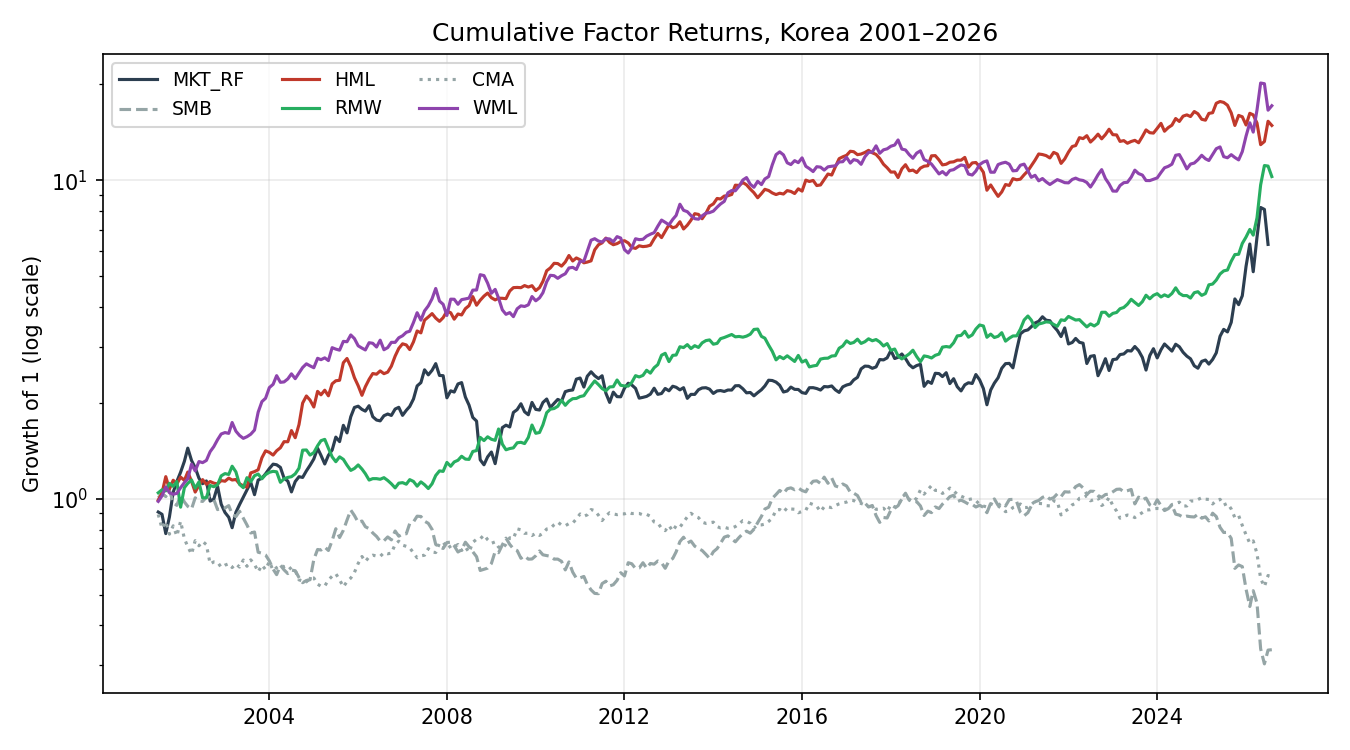
\includegraphics[width=0.9\textwidth]{figures/fig1_cumulative.png}
\caption{Cumulative factor returns, 2001--2026 (log scale).}
\label{fig:cumulative}
\end{figure}

Four stylized facts stand out. \emph{First}, the value premium is large and reliable (HML $+0.98$\%, $t=4.07$)---roughly twice recent US magnitudes---consistent with longstanding evidence that value works well in Korea and with the ``Korea discount'' discussion. \emph{Second}, profitability also earns a premium ($+0.86$\%, $t=3.55$) that exceeds typical US estimates of around $0.25$\%. \emph{Third}, the size premium has the wrong sign: small stocks \emph{underperformed} large stocks by 25 basis points per month on average, though not significantly. \emph{Fourth}, the investment factor is economically and statistically nil, as in many non-US markets. Internal factor correlations match FF stylized facts in direction: HML--CMA $+0.22$, RMW--SMB $-0.42$, RMW--CMA $-0.52$.

Momentum deserves its own paragraph because the Korean literature long held that it did not exist, based on pre-2000 samples \citep{griffin2003}. In this 2001--2026 sample WML earns $+1.04$\% per month ($t=4.12$). Three checks argue this is genuine rather than a construction artifact. Subperiod means decline from $+1.55$\% ($t=3.64$) in 2001--2010 to $+0.68$\% ($t=2.16$) in 2011--2020 and $+0.78$\% ($t=1.20$) after 2021, a decay profile familiar from the factor-publication literature \citep{mclean2016}. The size split shows stable small-stock momentum ($+0.98$\%, $t=4.78$) alongside noisier large-stock momentum ($+1.09$\%, $t=2.79$), matching prior Korean evidence that momentum weakens among the largest stocks. And the series co-moves sensibly with the French Emerging Markets momentum factor (correlation 0.58; means $+1.09$ vs.\ $+0.88$\%/month), of which Korea is a major constituent.

\subsection{Validation}

Three validation exercises support the series' accuracy (Figure~\ref{fig:validation} illustrates the first). The library's market return tracks the KOSPI index with a correlation of 0.994 and regression slope 0.985---not 1.0 by construction, since the library market is total-return and includes KOSDAQ while the index is a price index of the main board. Event months behave as they must: October 2008 ($-24.4$\% excess return), March 2020 ($-11.0$\%), April 2020 ($+11.3$\%), and the July 2026 crash, where the library's $-22.1$\% market return matches the KOSPI's $-22.2$\% within a decimal. Finally, against the French Asia-Pacific-ex-Japan factors, the market factor correlates at 0.65---the highest of all factor pairs, as it should be for a single country against a regional aggregate---while style-factor correlations are low (0.04--0.17), consistent with the well-documented local nature of characteristic factors.

\begin{figure}[ht]
\centering
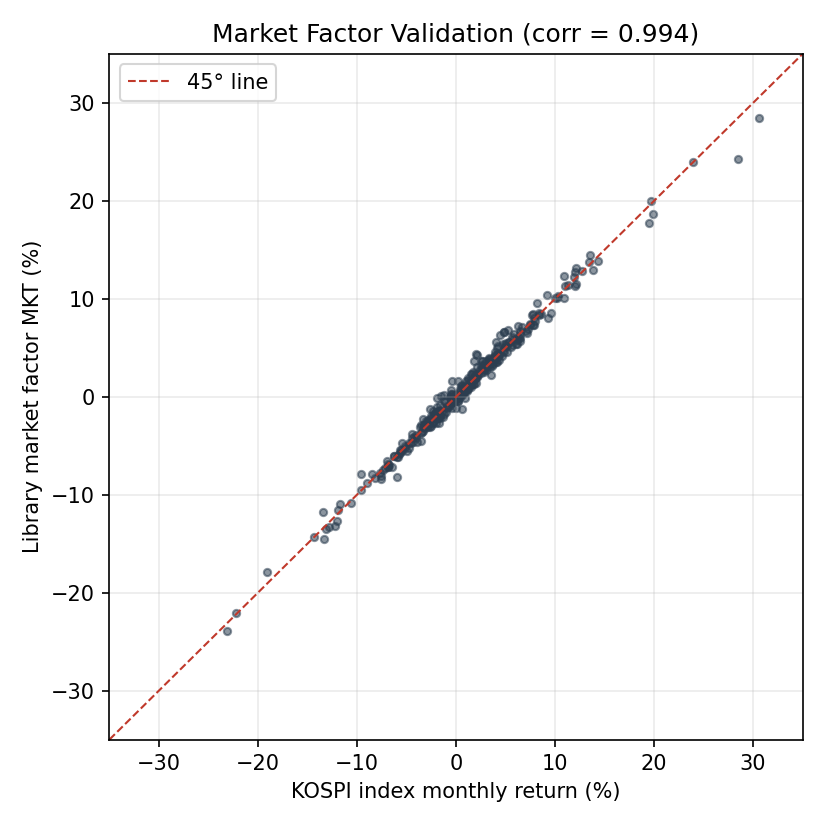
\includegraphics[width=0.55\textwidth]{figures/fig2_market_validation.png}
\caption{Library market factor versus KOSPI index monthly returns, 2001--2026.}
\label{fig:validation}
\end{figure}

\section{Usage, Citation, and Updates}\label{sec:usage}

\subsection{Access and formats}

The data ship as a single CSV (\texttt{data/factors\_monthly\_kr\_ff5.csv}) with columns \texttt{MKT\_RF, SMB, HML, RMW, CMA, WML, RF, MKT}, in percent per month, loadable in one line of Python or R; the repository includes worked examples, among them a Fama--MacBeth exercise for teaching. All construction code, the US replication test, the methodology note, the compliance matrix, and the validation report are in the same repository, \url{https://github.com/jihwanw/korea-fama-french-factors-}.

\subsection{Citation and versioning}

Each monthly release is archived on Zenodo with its own version DOI; the concept DOI (10.5281/\allowbreak zenodo.\allowbreak 22059320) always resolves to the latest version. General citations should use the concept DOI; studies for which exact reproducibility matters should cite the version DOI of the release actually used. This addresses a quiet problem with living datasets---that ``the data'' cited in a paper may have changed by the time a reader downloads it.

\subsection{Update protocol and revisions}

An automated job runs on the second day of each month, after month-end prices and the CD rate become available, rebuilding the full history from current vendor data rather than appending increments; restatements in the source data therefore propagate, and users should expect small historical revisions between versions (another reason version DOIs matter). The market and risk-free columns can lag one month pending the central bank's CD release.

\subsection{Limitations}

The factors are academic constructs, not investable strategies: they ignore transaction costs, short-sale constraints, and the illiquidity of the small-stock legs. The CMA factor is insignificant in Korea and should be interpreted accordingly. The delisting adjustment is an approximation, bounded above by the $-100$\% sensitivity check. Book equity omits the deferred-tax add-back. Finally, while the aggregated factors are freely redistributable, reproducing them from raw data requires the user's own WRDS license.

\section{Conclusion}\label{sec:conclusion}

This library lowers the fixed cost of Korean asset-pricing research from ``rebuild the factors'' to ``download a CSV,'' and it does so with a construction pipeline whose validity is demonstrated by US replication rather than asserted. The documented Korean landscape---strong value and profitability, inverted size, absent investment, post-2000 momentum---offers ready-made puzzles; companion work examines the July 2026 momentum crash visible in the series' final months. Contributions, corrections, and issue reports through the repository are welcome.

\begin{thebibliography}{9}

\bibitem[Barroso and Santa-Clara(2015)]{barroso2015}
Barroso, P., and P. Santa-Clara. 2015. Momentum has its moments. \emph{Journal of Financial Economics} 116:111--120.

\bibitem[Daniel and Moskowitz(2016)]{daniel2016}
Daniel, K., and T. Moskowitz. 2016. Momentum crashes. \emph{Journal of Financial Economics} 122:221--247.

\bibitem[Fama and French(1993)]{fama1993}
Fama, E. F., and K. R. French. 1993. Common risk factors in the returns on stocks and bonds. \emph{Journal of Financial Economics} 33:3--56.

\bibitem[Fama and French(2015)]{fama2015}
Fama, E. F., and K. R. French. 2015. A five-factor asset pricing model. \emph{Journal of Financial Economics} 116:1--22.

\bibitem[Fama and French(2017)]{fama2017}
Fama, E. F., and K. R. French. 2017. International tests of a five-factor asset pricing model. \emph{Journal of Financial Economics} 123:441--463.

\bibitem[Griffin et al.(2003)]{griffin2003}
Griffin, J. M., X. Ji, and J. S. Martin. 2003. Momentum investing and business cycle risk: Evidence from pole to pole. \emph{Journal of Finance} 58:2515--2547.

\bibitem[Jegadeesh and Titman(1993)]{jegadeesh1993}
Jegadeesh, N., and S. Titman. 1993. Returns to buying winners and selling losers: Implications for stock market efficiency. \emph{Journal of Finance} 48:65--91.

\bibitem[McLean and Pontiff(2016)]{mclean2016}
McLean, R. D., and J. Pontiff. 2016. Does academic research destroy stock return predictability? \emph{Journal of Finance} 71:5--32.

\bibitem[Shumway(1997)]{shumway1997}
Shumway, T. 1997. The delisting bias in CRSP data. \emph{Journal of Finance} 52:327--340.

\end{thebibliography}

\end{document}
